\documentclass[class=report,crop=false, 12pt]{standalone}
\usepackage[screen]{../myscratch}

\begin{document}


\titre[E]{Coordonnées $x,y$}
%===============================


\begin{enigme}

\textbf{Question.} Quel nombre à deux chiffres se cache sous le dessin suivant ?

\emph{Premier chiffre.} 
Ligne brisée qui relie les points de coordonnées :
$$(27,117) \quad (83,115) \quad (79,59) \quad (25,57) \quad (23,7) \quad (77,5)$$ 


\emph{Second chiffre.}
Ligne brisée qui relie les points de coordonnées :
$$(117,57) \quad (169,59) \quad (167,5) \quad (113,7) \quad (119,117) \quad (171,115)$$ 

%\begin{solution}
%Réponse : le nombre est $26$.
%\end{solution}

\end{enigme}



\begin{enigme}

Scratch part d'un point de coordonnées $(0,y)$ et se déplace vers la droite avec un angle de $95$\textdegree\ par rapport au Nord. Il rebondit une fois à droite puis une fois à gauche sur les bords de l'écran.

\myfigure{1}{
\small\tikzinput{coord3}
}  

\textbf{Question.} Quelle doit être la valeur de l'entier positif $y$ pour que Scratch repasse par l'origine $(0,0)$ après deux rebonds ?

\bigskip

\begin{center}
  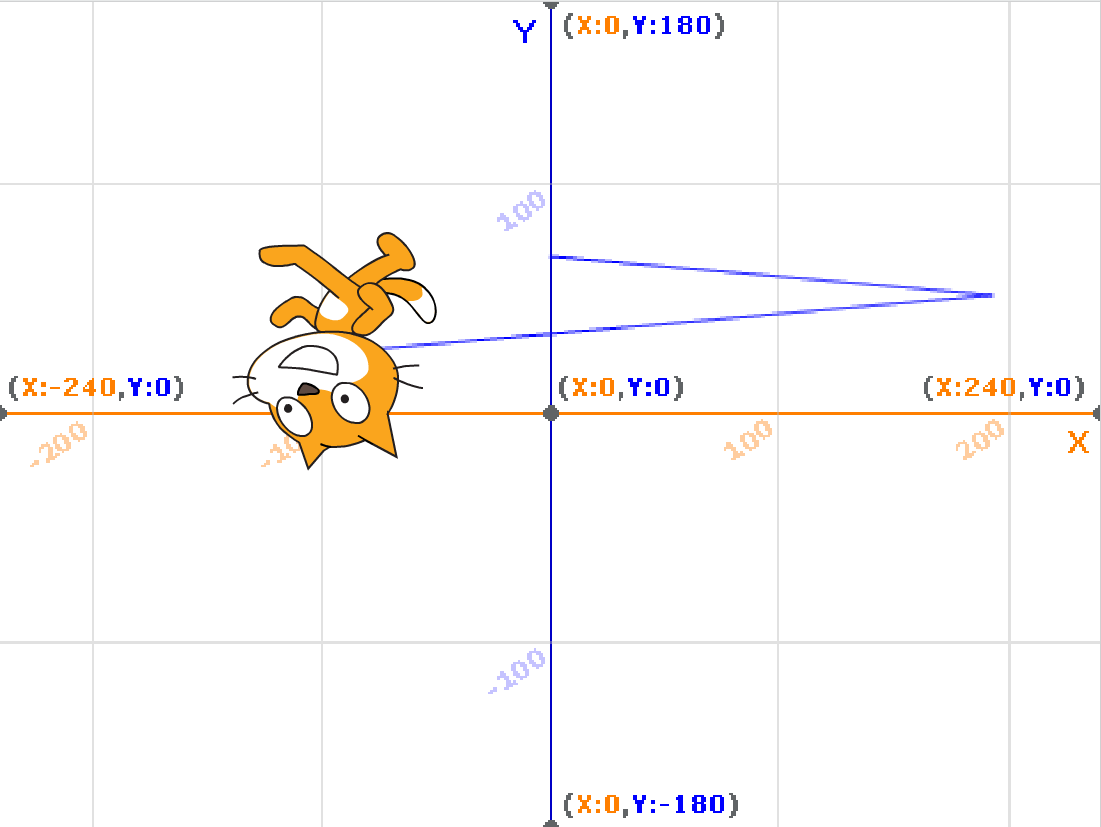
\includegraphics[width=0.6\textwidth]{ecran-03-eg2}   
\end{center}

\bigskip

\emph{Indications.} 
\begin{itemize}
  \item Utiliser comme arrière-plan la grille des coordonnées.
  
  \item Ne pas changer le costume Scratch par défaut.
  
  \item Faire avancer Scratch d'un seul pas à chaque fois et utiliser le bloc \og{}Rebondir si le bord est atteint\fg{}.
  
  \item Dans le menu \og{}Modifier\fg{}, il existe une fonction \og{}Activer le mode turbo\fg{} pour avancer plus vite.
  
  \item Une erreur de plus ou moins $2$ est acceptée !
\end{itemize}


%\begin{solution}
%Réponse : l'abscisse est environ $69$ ; les réponses valides sont donc $67,68,69,70,71$.
%\end{solution}

\end{enigme}



\begin{enigme}


On a associé une lettre à chaque zone de coordonnées.


\myfigure{0.70}{
\small\tikzinput{coord4}
}  

Scratch va se déplacer sur ce quadrillage. À chaque fin d'étape, la case sur laquelle il se trouvera contient une lettre du mot qui est à découvrir.
%Il faut deviner un mot en trouvant une par une les lettres qui le compose.

\begin{itemize}
  \item On part de $(0,0)$.
  \item \emph{Lettre 1.} S'orienter à $135$\textdegree\ et avancer de $200$.
  \item \emph{Lettre 2.} Conserver la même valeur pour $x$, mais avec $y=50$.
  \item \emph{Lettre 3.} Conserver la même valeur pour $y$, mais avec $x=-150$.
  \item \emph{Lettre 4.} Échanger $x$ et $y$ (partant du point $(x,y)$ il faut aller au point $(y,x)$).
  \item \emph{Lettre 5.} Ajouter $300$ à la valeur de $y$.
  \item \emph{Lettre 6.} Changer $x$ en $-x$.  
\end{itemize}


\bigskip

\textbf{Question.} Quel est ce mot ? Tu peux te renseigner sur la vie et l'activité scientifique de cette personne.



%\begin{solution}
%Réponse : le nom à trouver est \mot{TURING}.
%\end{solution}

\end{enigme}
\end{document}



